%PIP-412035RC020
\documentclass[rc]{physicsinprogress}

\pipvolume{2}
\pipissuedate{Feb. 2026}

\usepackage{siunitx}

\begin{document}




\title{Riding the wave: determining laser wavelength using a Michelson interferometer}
\author{Brookelyn H. Velmont}
\affiliation{%
Department of Physics and Astronomy,  Carthage College, 2001 Alford Park Drive, Kenosha, WI 53140, USA
}%
\pipdates{January 29, 2026}{February 5, 2026}
\begin{abstract}
 The wavelength of a helium-neon gas laser was determined using a Michelson interferometer by relating mirror displacement to interference fringe shifts. As the movable mirror was displaced, the number of fringe shifts $m$ was counted and the corresponding mirror displacement $d$ was recorded. Plotting $d$ as a function of $m$ revealed a linear relationship, where the slope corresponds to half the wavelength of the light, $d/m = \lambda/2$. Using this result, the wavelength was determined to be $\lambda$ = \num{653 \pm 6}nm.
\end{abstract}

\maketitle

\section{Introduction}
Michelson interferometers have been key components in many scientific applications, ranging from optical calibration on an optics table, to measuring the diameter of stars in stellar interferometry. The behavior of light was heavily debated with Isaac Newton proposing that light consists of many minute particles, while Christiaan Huygens argued that light behaved as a wave \cite{crew1900wave}. This debate persisted until Thomas Young's double-slit experiment provided strong evidence for the wave nature of light through the observation of interference patterns \cite{young1804bakerian}.

Interference patterns were crucial in proving light as a wave phenomenon. When two coherent light beams overlap, their relative phase determines whether they interfere constructively or destructively, producing a pattern of dark and bright fringes. In a Michelson interferometer this relative phase depends on the optical path difference between the two beams. By moving one of the mirrors the path difference changes in a controlled manner, causing the interference fringes to shift. By counting the number of fringes that pass a fixed reference point as the mirror is displaced, the wavelength of the light can be determined. The Michelson interferometer was developed by Albert A. Michelson to measure small differences in optical path length with extreme precision \cite{michelson1887art}. Michelson interferometry remains a foundational technique in modern physics, with applications ranging from precision metrology to gravitational wave detection.

\section{Key Findings}
The relationship between mirror displacement and fringe shifts stems from classical wave optics, where the phase of a light depends on its optical path length. In a Michelson interferometer (Fig. \ref{fig:drawing}.), light from a laser is divided by a beam-splitter into two beams that propagate along perpendicular arms. One beam travels to a fixed mirror, while the other travels to a movable mirror. The reflected beams return to the beam-splitter, where they recombine and produce an interference pattern at a viewing screen. When one mirror in the interferometer is moved by a distance $d$, the optical path length changes by $2d$, since the beam travels to the mirror and back. This change in path length alters the relative phase between the two beams, creating the predictable fringe pattern.

Each time the optical path length changes by one wavelength one fringe shift is observed. Measuring the mirror displacement over a known number of fringes therefore yields a linear relationship: 
\begin{equation}
\lambda = \frac{2d}{m}, 
\end{equation}
where $\lambda$ is the wavelength, $d$ is the mirror displacement, and $m$ is the number of oberved fringes.

The experiment used a PASCO OS-8514 helium-neon gas laser and a PASCO scientific Model OS-8501 interferometer consisting of a beam-splitter, a stationary mirror (M1), a moveable mirror (M2), and a viewing screen as shown in Fig.\ref{fig:drawing}. The laser was mounted on an optics bench, with the interferometer positioned approximately 20 centimeters away. The beam-splitter was oriented at \SI{45}{\degree} to direct light toward the stationary mirror, while the moveable mirror faced the laser. The viewing screen was placed behind the beam-splitter to oberve the interference pattern.
\begin{figure}
    \centering
    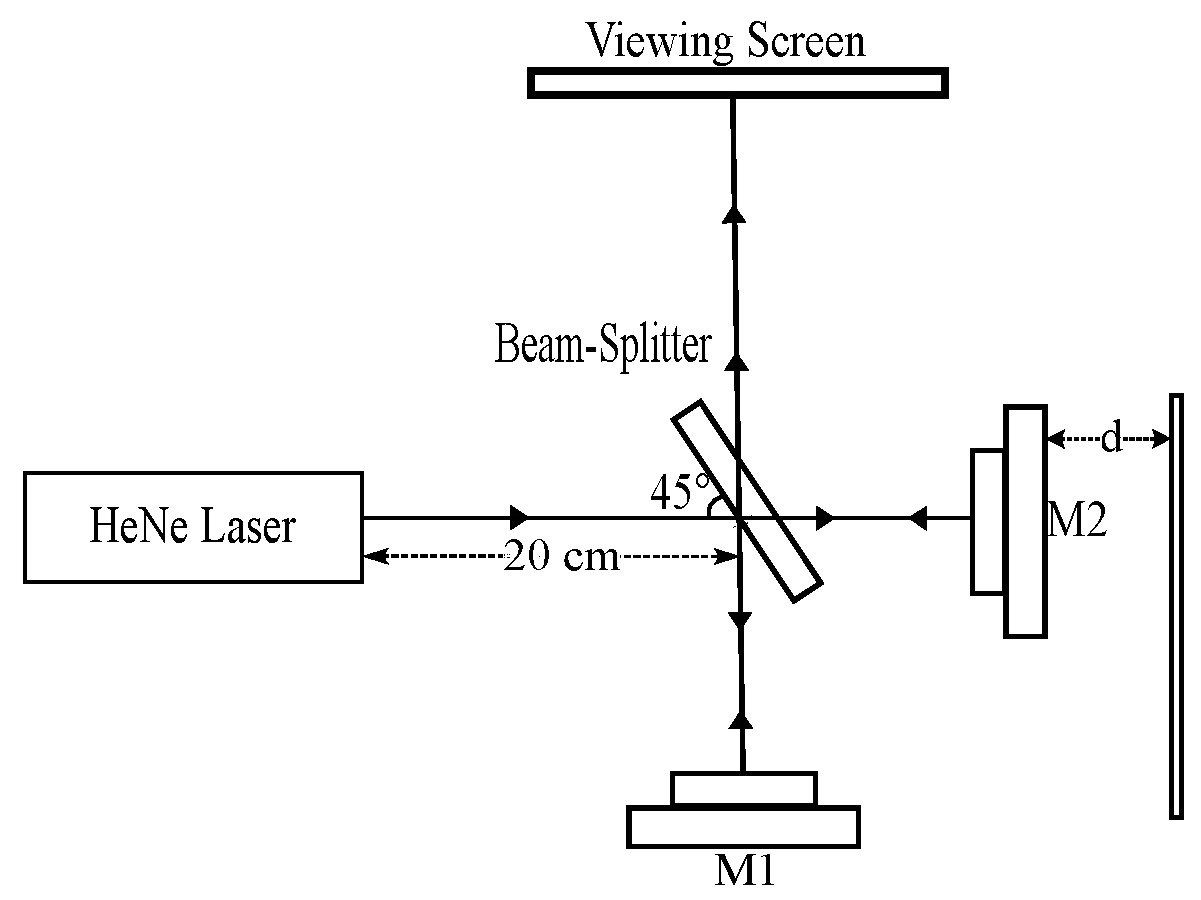
\includegraphics[ width=0.9\linewidth] {interferometer.pdf}
    \caption{A schematic of the Michelson interferometer used in this experiment. Light from a helium–neon laser is split by a beam-splitter and reflected by a stationary mirror (M1) and a movable mirror (M2). The two beams recombine at the beam splitter and form an interference pattern on the viewing screen. Displacement, $d$, of mirror M2 changes the optical path difference between the beams.}
    \label{fig:drawing}
\end{figure}

After aligning the interferometer to produce a clear circular fringe pattern as shown in Fig.\ref{fig:fringes}., data was collected by counting a predetermined number of fringes while measuring the corresponding displacement of mirror M2 using a micrometer. A fringe shift occurs when the optical path length of one arm changes, by moving M2, forcing the interference pattern to rearrange. The circular pattern in Fig.\ref{fig:fringes}. is due to M1 and M2 being parallel, and a shift causes the rings to expand or contract. A single fringe shift is counted from the center of one dark ring to the next. An error for the distance measured was estimated to be $\delta =\SI{0.5}{\micro\metre}$ = \SI{500}{nm} because the micrometer was marked in increments of one micrometer, making it hard to exactly distinguish an exact measurement. A mechanical band ensured that M2 remained parallel with M1 while being moved. Measurements began with 20 fringes and increased in increments of 5 up to 70 fringes. Measuring larger numbers of fringes reduced the relative uncertainty in the wavelength calculation.
\begin{figure}
    \centering
    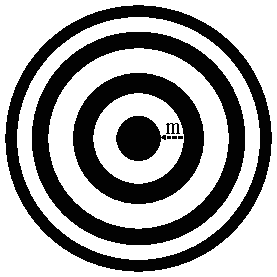
\includegraphics[ width=0.55\linewidth] {fringes.pdf}
    \caption{Interference fringe pattern observed on the viewing screen after alignment of the Michelson interferometer. Bright and dark circular fringes result from constructive and destructive interference of the two coherent beams. Fringe shifts, $m$, were counted as mirror M2 was displaced.}
    \label{fig:fringes}
\end{figure}
\begin{figure}
    \centering
    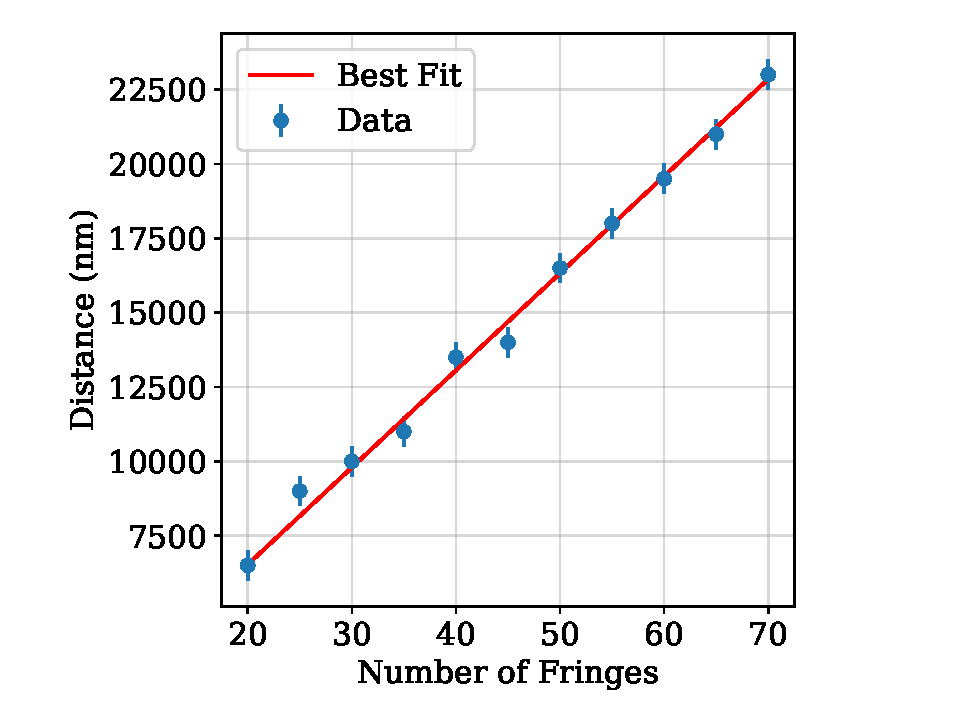
\includegraphics[ width=1.0\linewidth] {slopeiswavelength.pdf}
    \caption{Mirror displacement as a function of fringe count for a HeNe laser. A least squares linear fit with the y-intercept constrained to zero was applied to the data, yielding a slope of $M$ = 326 $\pm$ 3 nm/fringe.} 
    \label{fig:slope}
\end{figure}

The wavelength of the helium-neon laser was determined by measuring the mirror displacement required to produce a known number of interference fringe shifts. Mirror displacement was plotted as a function of fringe count as seen in Fig.\ref{fig:slope}. There is a clear linear relationship between the two, indicating that the mirror displacement increased proportionally with the number of oberved fringes. The linear relationship observed is expected from the theoretical prediction that the mirror displacement is proportional to the number of fringe shifts. In Fig.\ref{fig:slope}., the y-intercept is constrained to the origin, $(0,0)$, due to the experimental setup in which distance is measured as a function of the number of fringes. Therefore, if zero fringe shifts have occurred, the measured distance is zero.

A linear fit to the data yielded a slope corresponding to half the wavelength of the light source. Using this slope, the wavelength of the laser was determined to be 
\begin{equation}
\lambda = \frac{2d}{m} = \SI{653 \pm 6}{\nm}.
\end{equation}
The primary source of uncertainty stemmed from the measured distance of the mirror displacement. Because fringes are discrete and easily counted, uncertainty in fringe number was negligible compared to uncertainty in the measured mirror displacement. The measured wavelength was consistent with the true wavelength value of a helium-neon gas laser of $\lambda = \SI{632.8}{nm}$ \cite{pasco_mini_laser}.

\section{Conclusion}
The wavelength of the helium-neon laser was successfully determined using a Michelson interferometer by relating mirror displacements to interference fringe shifts. The measured value corresponds to a z-score of 3.19 when compared to the expected wavelength, which gives a two-tailed p-value of approximately 0.0014. This indicates that the measured wavelength differs from the expected value by over three standard deviations, making the difference statistically significant. The accuracy of the measurement was primarily limited by uncertainty in the mirror displacement. The micrometer was marked in increments of one micrometer, making it hard to exactly distinguish an exact measurement between a \SI{0.5}{\micro\metre} increment. This difficulty in exact measurement is how the error for distance measured was estimated to be $\delta = \SI{0.5}{\micro\metre}$ \= 500 nm. Future measurements could reduce these effects by using automated fringe detection or larger mirror displacements. 

\begin{acknowledgments}
This research would not have been made possible without funding from the Carthage College Physics and Astronomy Department along with assistance from Dr. Joseph Anderson.
\end{acknowledgments}

\section*{Data Availability Statement}
A Jupyter notebook containing all the experimental data, data analysis, figure generation, and additional information on uncertainty analysis can be found in the supplemental materials. \footnote{See online article posting for access to supplemental material.}

\bibliography{bib.bib}

\end{document}
